\section{Durchführung}
Zum Versuchsaufbau gehört eine optische Bank, auf der Reiter mit verschiedenen optischen Elementen bewegt werden können. Zu den Elementen gehören eine Halogenlampe als Lichtquelle, Linsen unterschiedlicher Brennweite, ein Schirm,
der Gegenstand 'Perl L' und zwei Filter in den Farben Rot und Blau. Der Versuch unterteilt sich in drei Teile, in denen auf unterschiedliche Weise die Brennweite der verwendeten Linse bestimmt werden soll.

\subsection{Bestimmung der Brennweite durch Messung der Gegenstandsweite und der Bildweite}
Zunächst werden die Lampe, das 'Perl L', eine Sammellinse bekannter Brennwerte und ein Schirm auf der Bank platziert. Dann wird eine bestimmte Gegenstandsweite $g$ festgelegt und der Schirm so verschoben, bis auf diesem das 
Bild von 'Perl L' scharf zu erkennen ist. Auf diese Weise werden für mindestens 10 eingestellte Gegenstandsweiten $g$ die zugehörige Bildweite $b$ ausgemessen und notiert, wodurch die Brennweite der Linse bestimmt und mit der
vom Hersteller angegebenen Brennweite verglichen werden kann.


\subsection{Bestimmung der Brennweite einer Linse nach der Methode von Bessel}
Im zweiten Versuchsteil soll die Brennweite der Linse mit der Methode von Bessel bestimmt werden. Dazu wird ein fester Abstand $e$ zwischen Gegenstand und Bild eingestellt, zwischen denen an zwei Stellen ein scharfes Bild auf dem 
Schirm zu erkennen ist. An diesen Positionen werden die Gegenstands- und Bildweiten $g_1$ und $b_1$, bzw. $g_2$ und $b_2$ gemessen und notiert. Die Messung wird dann für mindestens neun weitere Abstände $e_{\text{i}}$ durchgeführt.

Danach wird ein roter oder blauer Filter vor das 'Perl L' gesetzt. Für diesen Aufbau werden auf dieselbe Weise fünf weitere Messungen gemacht, woraufhin der Filter ausgewechselt wird und wiederum fünf mal Wertepaare notiert werden.

\begin{figure}[h!tbp]
	\centering
	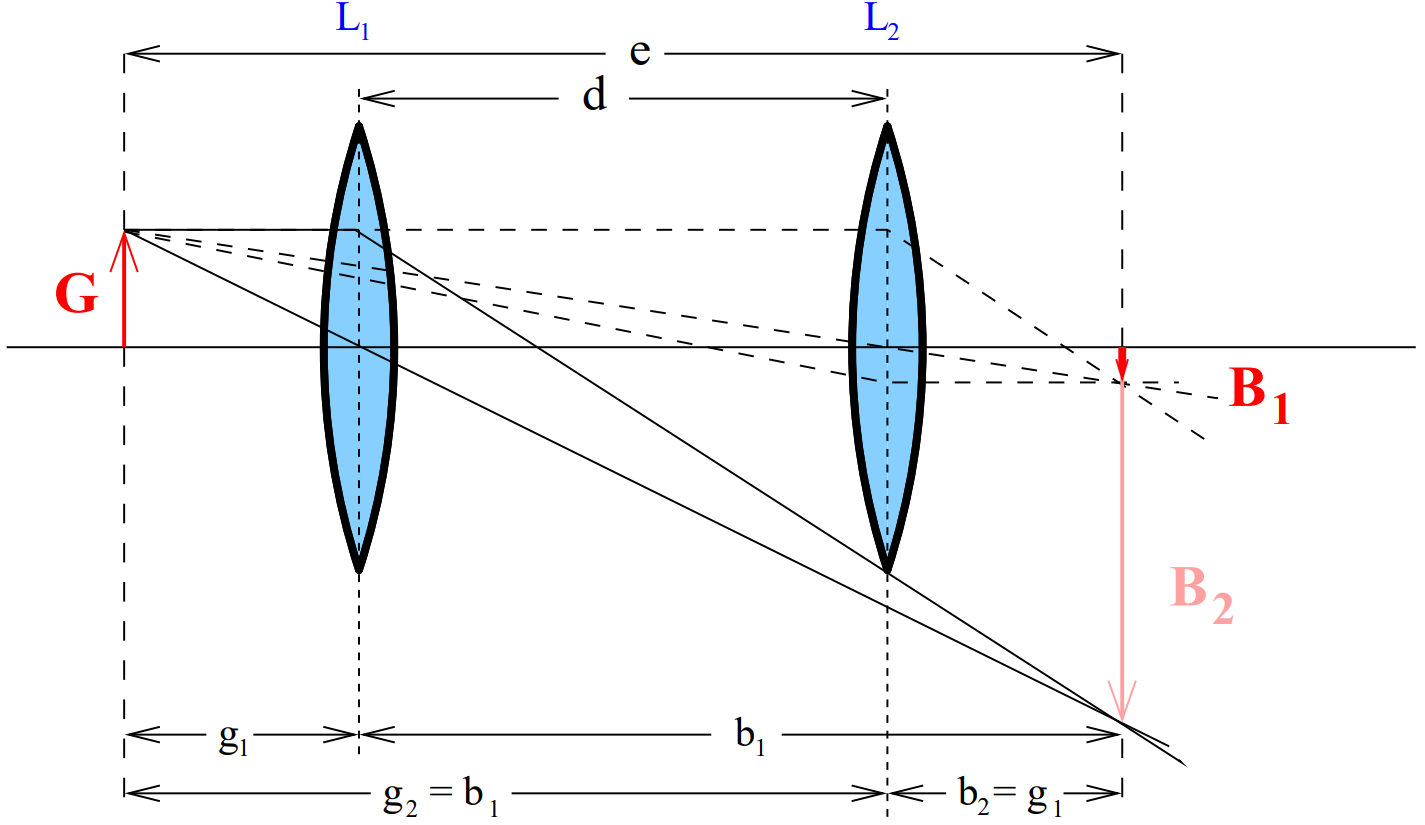
\includegraphics[width=0.6\linewidth]{aufbau1.png}
	\caption{Versuchsaufbau zur Methode nach Bessel.\cite[4]{anleitung408}}
	\label{fig:aufbau1}
\end{figure}


\section{Bestimmung der Brennweite eines Linsensystems nach der Methode von Abbe}
Im letzten Versuchsteil erfolgt die Bestimmung der Brennweite mit der Methode nach Abbe. Dazu wird zusätzlich eine Zerstreuunglinse eingesetzt, die die negative Brennweite der verwendeten Sammellinse besitzt. Die beiden Linsen 
werden dann so verschoben, dass sie sich berühren und werden im Laufe des Versuchs nicht mehr getrennt. Es wird dann ein Referenzpunkt $A$ festgelegt, der sich hier zwischen den beiden Linsen befindet. Von diesem Referenzpunkt 
aus werden die Abstände $g'$ und $b'$ zum 'Perl L' und zum Schirm gemessen, sowie auch der Abbildungsmaßstab $V$. Die prinzipielle Versuchsdurchführung gleicht der des ersten Teils. Es werden also zehn verschiedene Gegenstandsweite $g'$ 
festgelegt und die Bildweiten $b'$ dazu gemessen. Zusätzlich soll die Größe des 'Perl L' gemessen werden, sowie die Größe des Bildes bei jeder Messung.

\begin{figure}[h!tbp]
	\centering
	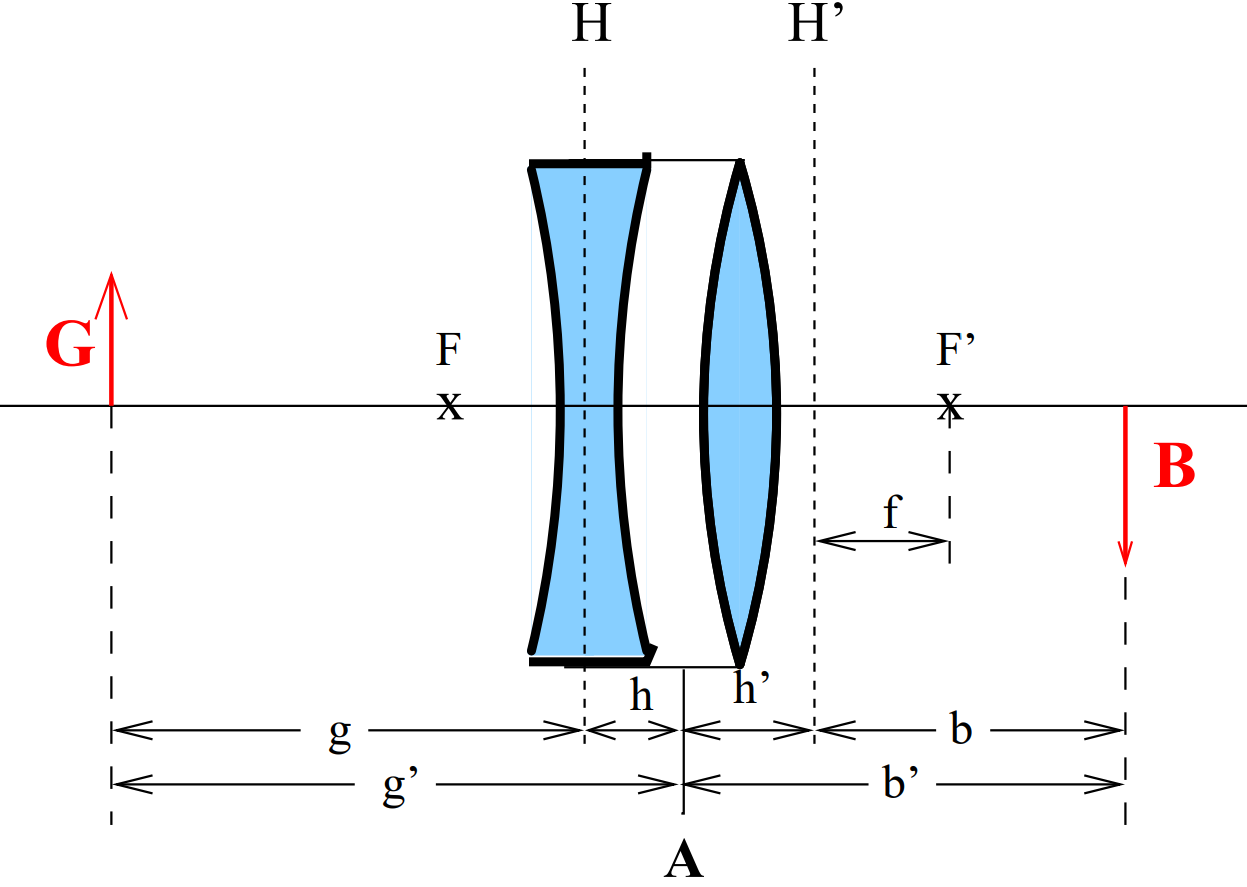
\includegraphics[width=0.6\linewidth]{aufbau2.png}
	\caption{Versuchsaufbau zur Methode nach Abbe.\cite[5]{anleitung408}}
	\label{fig:aufbau2}
\end{figure}

